\subsection{Introducción:}

En este ejercicio trabajaremos con todo lo relacionado a la \textit{TSS}, realizaremos los siguientes ítems:

\begin{itemize}



\item [\textit{a)}]  Definir las entradas en la GDT que considere necesarias para ser usadas como descriptores de \textit{TSS}.

\item [\textit{b)}] Completar la entrada de la \textit{TSS} de la tarea Idle con la información de la tarea Idle. La tarea Idle se encuentra en la dirección 0x00016000. La pila se alojará en la misma dirección que la pila del kernel y debe compartir el mismo CR3 que el kernel.

\item [\textit{c)}]  Construir una función que complete una TSS libre con los datos correspondientes. El código de las tareas se encuentra a partir de la dirección 0x00010000. Para la dirección de la pila se debe utilizar el mismo espacio de la tarea, la misma crecerá desde la base de la tarea. Para el mapa de memoria se debe construir uno nuevo utilizando la función \textit{mmu\_inicializar\_dir\_perro}. Además, tener en cuenta que cada tarea utilizará una pila distinta de nivel 0. 

\item [\textit{d)}] Completar la entrada de la GDT correspondiente a la tarea\_inicial.

\item [\textit{e)}]  Completar la entrada de la GDT correspondiente a la tarea Idle.

\item [\textit{f)}]  Escribir el código necesario para ejecutar la tarea Idle, es decir, saltar intercambiando las TSS, entre la tarea\_inicial y la tarea Idle.

\item [\textit{g)}] Modificar la rutina de la interrupción 0x46, para que implemente los servicios según se indica en la sección 4.4, sin desalojar a la tarea que realiza el syscall.

\item [\textit{h)}]  Ejecutar una tarea perro manualmente. Es decir, crearla y saltar a la entrada en la gdt de su respectiva TSS.

\end{itemize}

\subsection{Item a)}
Para este punto definimos 18 nuevas entradas en la gdt.\\
Las primeras dos nuevas entradas de la gdt corresponden a la \textit{Tarea inicial} y a la taréa \textit{idle} respectivamente. Las siguientes 8 entradas corresponden a los 8 perros del \textbf{jugador A} ordenadas en orden decreciente en el número de perros, es decir, el \textit{id}. Finalmente las últimas 8 entradas corresponden a los 8 perros del \textbf{jugador B} también ordenadas decrecientemente en el \textit{id}.\\

\subsection{Item b)}
Para este item lo que hacemos es lo siguiente:\\
Primero completamos el campo \textit{base} de la entrada de la gdt correspondiente a la taréa \textit{idle}.Para ello le asignamos la dirección 0x00016000 tal como indica el enunciado.\\
Como también nos dicen que comparte el \textit{esp} con el \textit{kernel} entonces en la entrada \textit{esp} de la \textit{TSS} le asigno 0x27000 que era el \textit{esp} asignado al kernel.Además como comparten el \textit{cr3} le asigno a la entrada correspondiente en la \textit{TSS} 0x28000.\\% por qué? ni idea
La siguiente figura muestra como queda la \textit{TSS}\\


INSERTAR IMAGEN


\subsection{item c)}
Lo que nos piden en este punto es hacer la función $void$ $tss\_completar(int$ $jugador, int$ $perro, perro\_t *rrope)$\\
Lo primero que  hago en esta función es pedir una nueva página libre para usarlo como una pila de nivel 0 para la taréa.\\
Lo siguiente que hago es preguntar si es la taréa (el perro) es una taréa correspondiente al \textbf{jugador A} o al \textbf{jugador B}. Supongamos que estoy rellenando una TSS para un perro del jugador A. Para el jugador B es similar.\\
En el campo esp0 pongo la nueva página que pedí. Va a ser su espacio de trabajo.\\
En los campos \textit{cs}, \textit{es}, \textit{gs}, \text{ss}, \textit{ds}, \textit{fs} tienen los segmentos definidos anteriormente en la gdt.\\
Las entradas \textit{esp} y \textit{ebp} tienen 0x0402000-12.\\
La entrada \textit{eip} tiene 0x00401000.\\
\textit{eeflags} = 0x202, ... y así rellenamos las otras entradas con los valores correspondientes.\\
Lo único distinto a lo descripto en el pdf es la entrada cr3 que va a ser distinto para cada taréa.\\
El nuevo cr3 va a ser el devuelto por la función mmu\_inicializar\_memoria\_perro. Se lo asigno al campo correspondiente y actualizo la entrada correspondiente a la GDT para esa taréa seteando los campos base e índice.
La siguiente imágen muestra dicho proceso.\	\

\subsection{item d)}

La entrada de la GDT correspondiente a la taréa inicial en principio la definimos con cualquier 
valor  en la base pero con los valores correspondientes en los demás campos.

\begin{figure}[H]
\begin{center}
\minipage{1.00\textwidth}
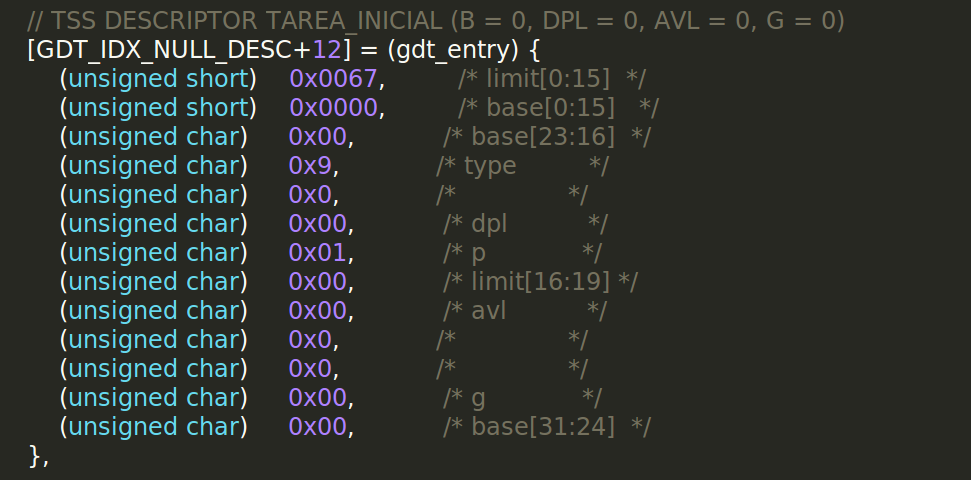
\includegraphics[width=\linewidth]{ejercicio6/gdt_tarea_inicial.png}
\caption{{\small \textit{Entrada de la GDT correspondiente a la tarea inicial }}}
\endminipage
\end{center}
\end{figure}


Luego con la función tss\_inicializar le asignamos la base correspondiente.

\begin{figure}[H]
\begin{center}
\minipage{1.00\textwidth}
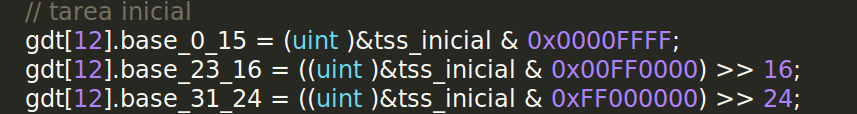
\includegraphics[width=\linewidth]{ejercicio6/tss_inicializar_base_inicial.png}
\caption{{\small \textit{Entrada de la GDT correspondiente a la tarea inicial }}}
\endminipage
\end{center}
\end{figure}

\subsection{item e)}
Esta sección es similar a la anterior. Creamos una entrada en la GDT para esta taréa y en la función tss\_inicializar seteamos los valores correspondientes para su base en la GDT y también seteamos su TSS.\\
Como nos dicen que la taréa se encuentra en la dirección 0x00010000 ese es el valor que ponemos en la base y por el enunciado va a compartir el CR3. Lo mismo con su pila.\\
\begin{figure}[H]
\begin{center}
\minipage{1.00\textwidth}
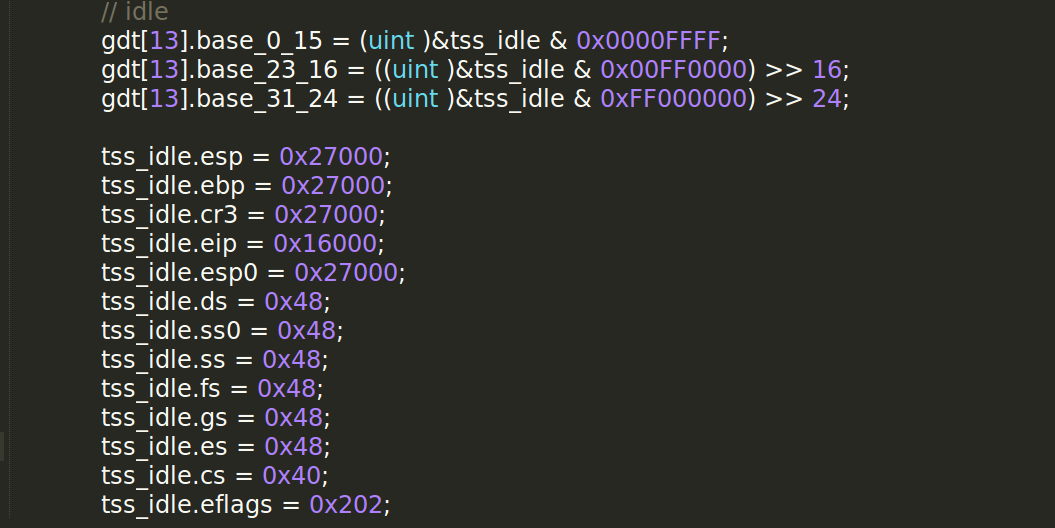
\includegraphics[width=\linewidth]{ejercicio6/tss_idle.png}
\caption{{\small \textit{Seteo la TSS de la tarea idle con los valores correspondientes}}}
\endminipage
\end{center}
\end{figure}

\subsection{item f)}
Esto es simplemente hacer un jump far en el archivo kernel.asm.\\
El intercambio en los valores de la TSS lo hace automáticamente el procesador.\\
 $jmp$ 0x68:0

 \subsection{item g)}
Para este punto lo que hacemos en la interrupción 0x46 es llamar a la función $game\_syscall\_manejar$ pasandole los parámetros que me llegan en la interrupción por EAX y ECX.\\
Y lo que hace la función es, dependiendo de los parámetros que le llega, llama a la función correspondiente ya séa:\\
$game\_perro\_mover$, $game\_perro\_cavar$ o $game\_perro\_olfatear$. El código es el siguiente:\\

\begin{figure}[H]
\begin{center}
\minipage{1.00\textwidth}
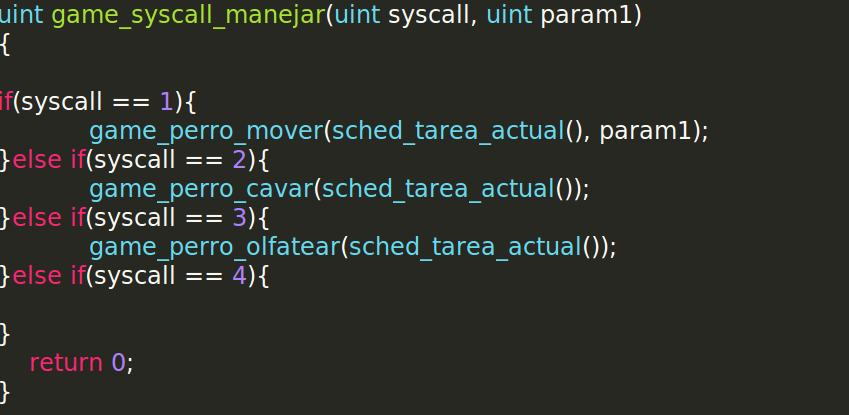
\includegraphics[width=\linewidth]{ejercicio6/syscall_manejar.png}
\caption{{\small \textit{Manejo de interrupciones}}}
\endminipage
\end{center}
\end{figure}

 \subsection{item h)}
 NO ESTÁ HECHO TODAVIA. VA A ESTAR EN kernel.asm